\documentclass[a4paper,12pt]{article}
\usepackage[utf8]{inputenc}
\usepackage[polish]{babel}
\usepackage[T1]{fontenc}
\usepackage{amsmath}
\usepackage{graphicx}
\usepackage{geometry}
\usepackage{float}
\usepackage{caption}
\usepackage{listings}
\usepackage{xcolor}
\usepackage{amssymb}
\usepackage{inconsolata}

\definecolor{bg}{RGB}{30,33,38}
\definecolor{fg}{RGB}{220,220,220}
\definecolor{comment}{RGB}{106,153,85}
\definecolor{keyword}{RGB}{86,156,214}
\definecolor{string}{RGB}{206,145,120}
\definecolor{number}{RGB}{181,206,168}
\definecolor{func}{RGB}{220,220,170}
\definecolor{linenumber}{RGB}{90,90,90}


\lstdefinestyle{vscodedark}{
    language=Python,
    backgroundcolor=\color{bg},
    basicstyle=\ttfamily\small\color{fg},
    keywordstyle=\color{keyword},
    commentstyle=\color{comment}\itshape,
    stringstyle=\color{string},
    numberstyle=\tiny\color{linenumber},
    numbers=left,
    numbersep=10pt,
    frame=none,
    breaklines=true,
    breakatwhitespace=true,
    showstringspaces=false,
    tabsize=4,
    keepspaces=true,
    xleftmargin=2em
}



\geometry{margin=2.5cm}

\title{
\Large Projektowanie Systemów Wizyjnych \\[6pt]
\textbf{Kalkulator bilonu}
}

\author{Piotr Sawicki 319003, Michał Piotrkowski 319001}
\date{Styczeń 2026}

\begin{document}

\maketitle

\section{Cel projektu}
Celem projektu było zaprojektowanie i implementacja systemu wizyjnego zdolnego do automatycznego wykrywania, identyfikacji oraz sumowania wartości polskich monet znajdujących się na zdjęciu. 

\section{Opis rozwiązania}
Ostateczna wersja systemu opiera się na bibliotece OpenCV i wykorzystuje dwuetapowy proces: manualną kalibrację skali oraz dynamiczną detekcję obiektów z wykorzystaniem transformaty Hougha.

\subsection{Metoda wyznaczania skali}
W toku prac zdecydowano się na uproszczenie interfejsu kalibracji. Użytkownik, po uruchomieniu programu, wskazuje na obrazie dwa punkty odpowiadające odcinkowi o długości \textbf{1 cm} (np. na linijce umieszczonej obok monet). 
Program oblicza dystans między punktami wykorzystując następujący wzór:
$$d_{px} = \sqrt{(x_2-x_1)^2 + (y_2-y_1)^2}$$
Na tej podstawie wyznaczany jest współczynnik $px\_per\_cm$, który służy do późniejszego przeliczania promienia wykrytych okręgów na rzeczywiste wymiary w milimetrach. Przyjęcie odcinka o znanej długości eliminuje wpływ zmiennej odległości aparatu od sceny, co stanowi kluczowy element zapewnienia poprawności dalszych obliczeń geometrycznych.

\subsection{Detekcja i klasyfikacja monet}
System rozpoznaje trzy wybrane nominały monet złotowych, charakteryzujące się relatywnie dużymi i łatwymi do rozróżnienia średnicami. Takie podejście umożliwia stabilną pracę algorytmu:
\begin{table}[H]
\caption{Parametry monet przyjęte w algorytmie.}
\centering
\begin{tabular}{|c|c|c|c|}
\hline
\textbf{Nominał} & \textbf{Średnica (mm)} & \textbf{Kolor oznaczenia} & \textbf{Wartość} \\ \hline
1 PLN & 23.0 & Magenta & 1.00 \\ \hline
2 PLN & 21.5 & Pomarańczowy & 2.00 \\ \hline
5 PLN & 24.0 & Czerwony & 5.00 \\ \hline
\end{tabular}
\end{table}

Klasyfikacja odbywa się poprzez porównanie obliczonej średnicy wykrytego okręgu z wzorcami. Jeśli różnica wynosi mniej niż 0.8 mm, moneta zostaje zakwalifikowana do danego nominału. W przeciwnym razie obiekt oznaczany jest symbolem "?".

\section{Preprocessing obrazu}
Najważniejszym etapem pracy jest odpowiednie przygotowanie obrazu do pracy z nim. W tym celu skorzystano z funkcji należących do biblioteki OpenCV. 

Wstępne przetwarzanie obrazu zaprojektowano jako wieloetapowy potok (pipeline), mający na celu maksymalizację stosunku sygnału do szumu. Po konwersji do skali szarości, kluczowym elementem było zastosowanie algorytmu CLAHE. W przeciwieństwie do globalnego wyrównywania histogramu, CLAHE zapobiega nadmiernemu wzmocnieniu szumu tła w jednolitych obszarach, co jest krytyczne przy analizie metalicznych, refleksyjnych powierzchni monet. Następnie obraz poddano filtracji filtrem Gaussa ($7 \times 7, \sigma=1.5$). Operacja ta pełni rolę filtra dolnoprzepustowego, usuwając teksturę podłoża i drobne zarysowania monet, które mogłyby generować fałszywe krawędzie w algorytmie Canny’ego, będącym wewnętrznym etapem transformaty Hougha.

Na zdjęciu~\ref{fig:pre} zaprezentowano poszczególne etapy działania preprocessinu, na ostatnim zdjęciu zaprezentowano w jaki sposób realizowane jest wykrywanie krawędzi metodą Canny'ego.

    \begin{figure}[H]
        \centering
        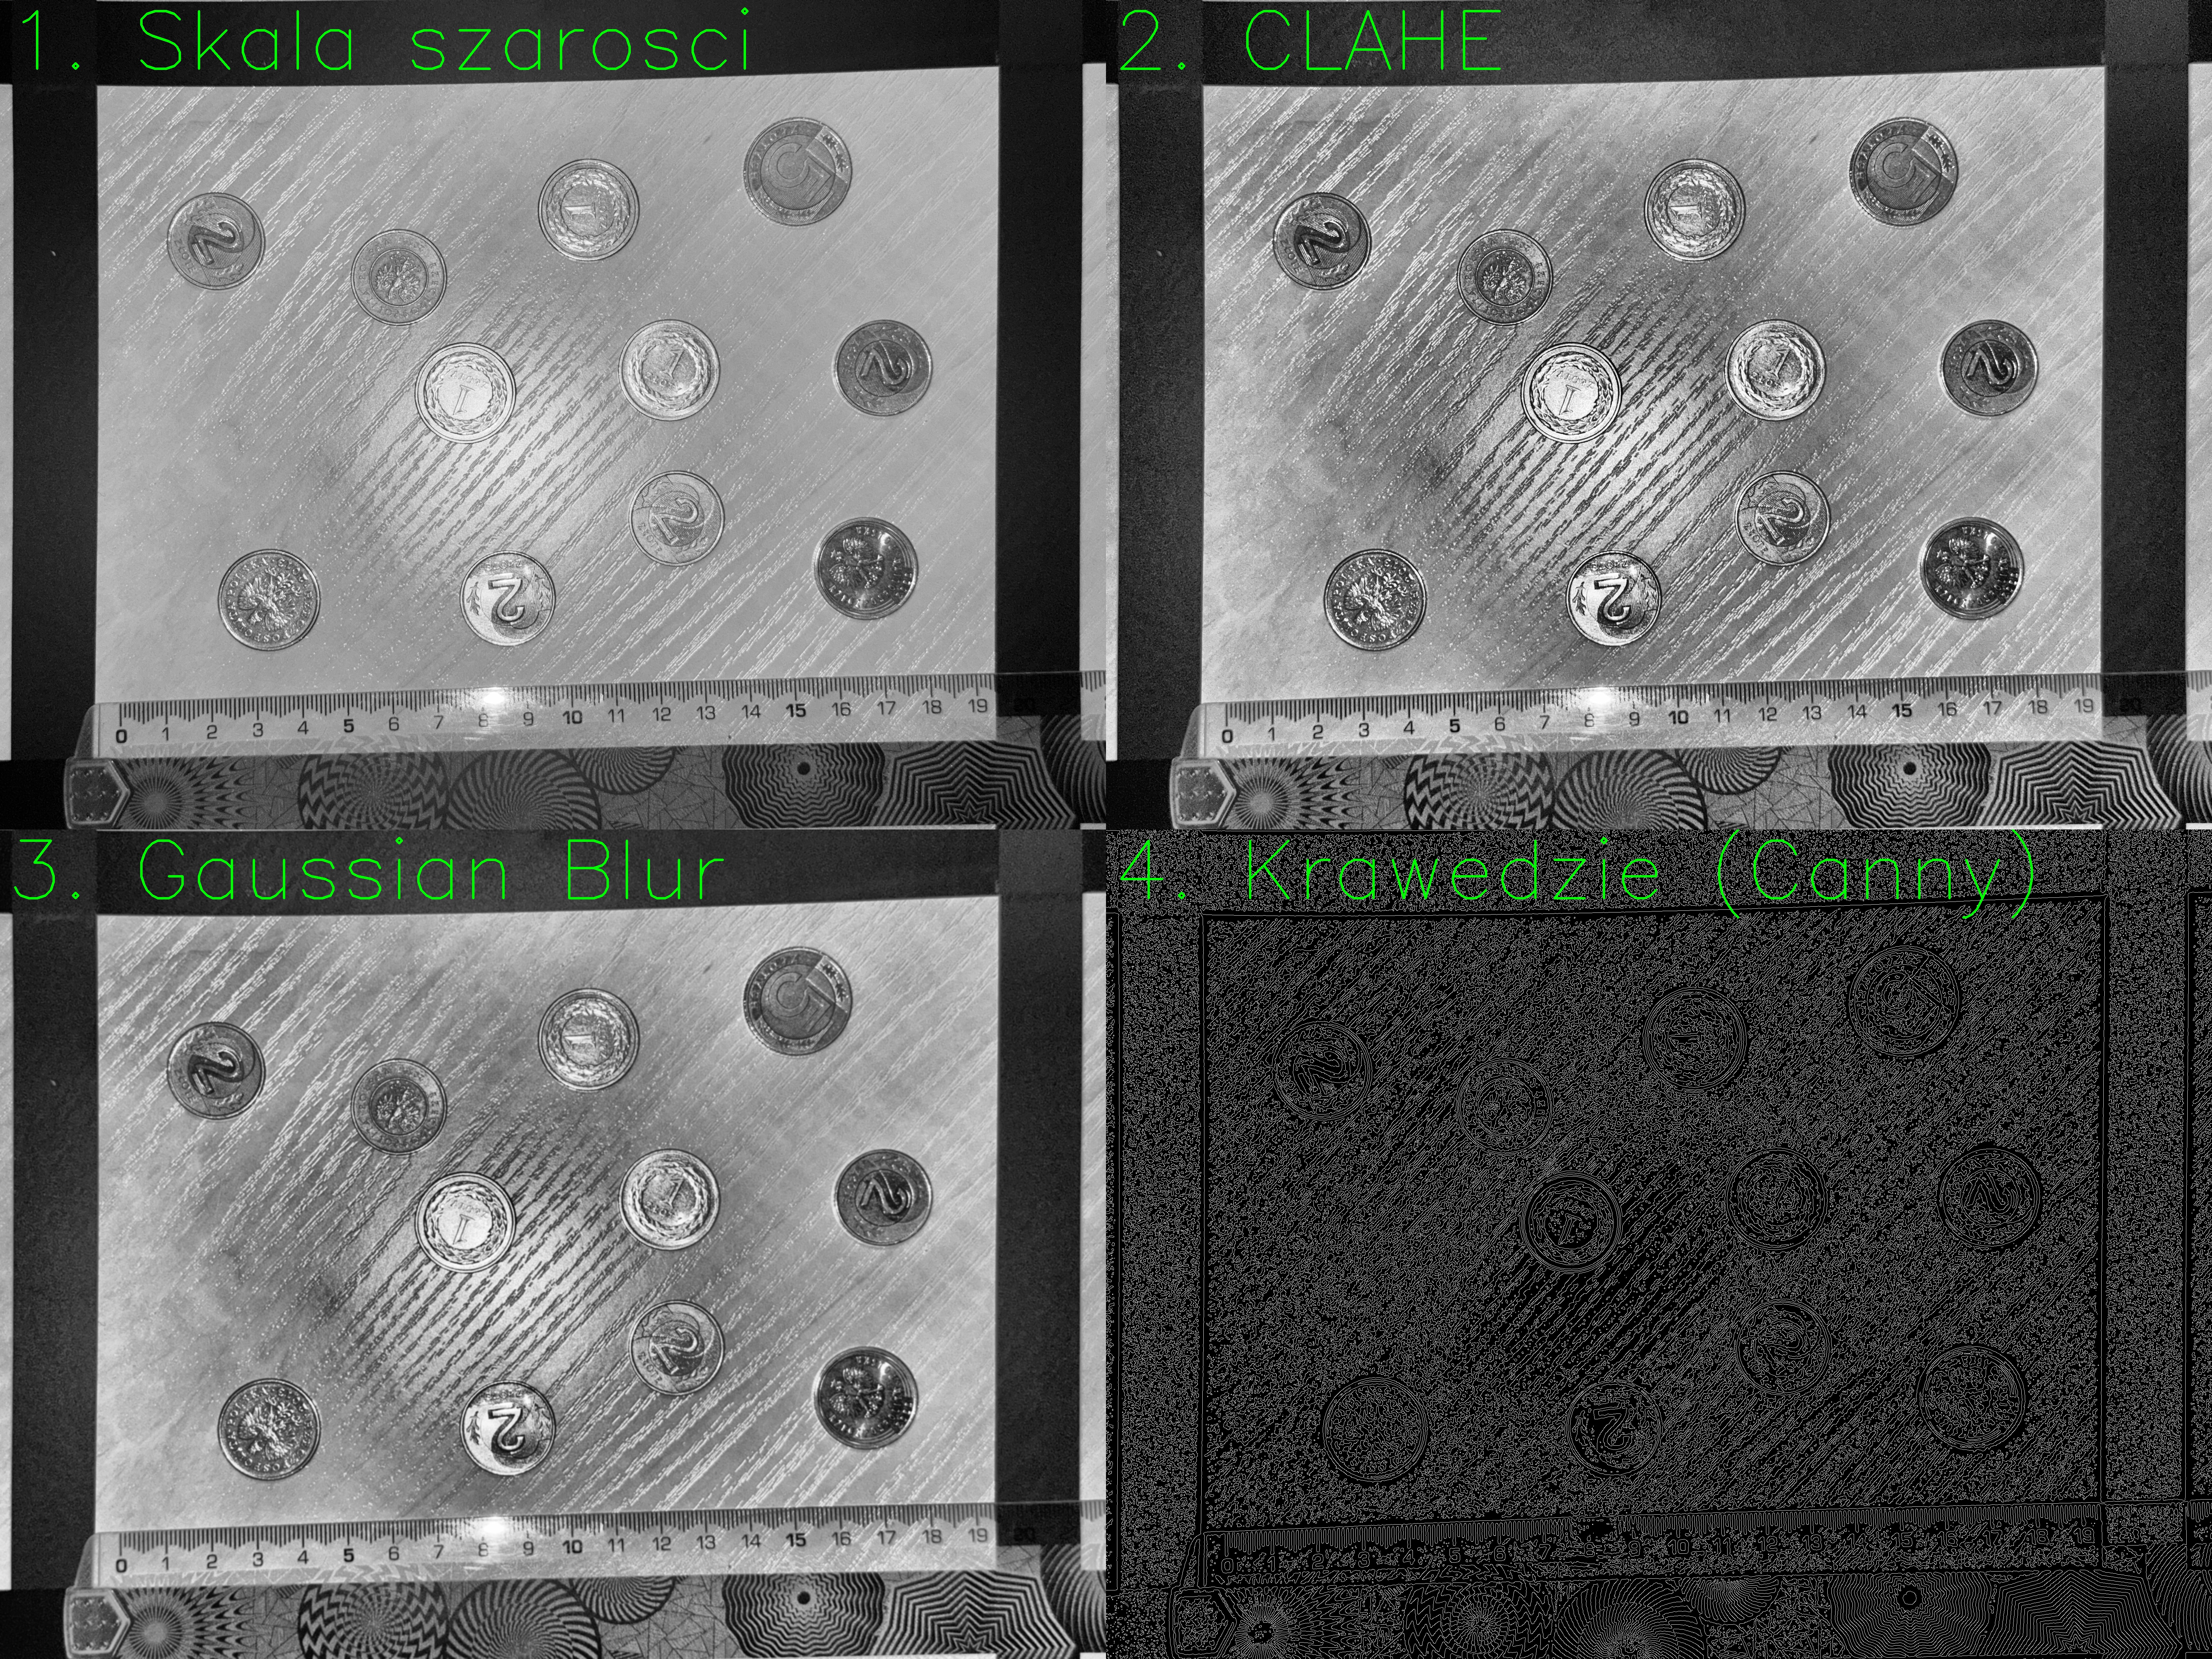
\includegraphics[page=1, width=0.9\textwidth, , trim= 0cm 0cm 0cm 0cm, clip]{wyniki/do_sprawozdania/preprocessing.jpg}
        \caption{Wizualizacja etapów wstępnego przetwarzania obrazu: od lewej górnej krawędzi – konwersja do skali szarości, lokalne wyrównanie histogramu (CLAHE), wygładzanie filtrem Gaussa oraz końcowa ekstrakcja krawędzi detektorem Canny’ego.}
        \label{fig:pre}
    \end{figure}


\section{Implementacja algorytmu}
Kluczowym elementem systemu jest moduł dynamicznego dostrajania parametrów funkcji \texttt{cv2.HoughCircles}. Dzięki zastosowaniu suwaków, użytkownik może w czasie rzeczywistym korygować:
\begin{itemize}
    \item \textbf{Param1:} próg dla detektora krawędzi Canny'ego.
    \item \textbf{Param2:} próg dla akumulatora centrów okręgów.
    \item \textbf{Minimalny dystans:} zapobiega nakładaniu się detekcji na jednej monecie.
    \item \textbf{Parametr dp:} rozdzielczość akumulatora.
\end{itemize}

    \begin{figure}[H]
        \centering
        \includegraphics[page=1, width=0.8\textwidth, , trim= 0cm 0cm 0cm 0cm, clip]{wyniki/do_sprawozdania/dzialanie_programu.png}
        \caption{Okno kalibracji}
        \label{fig:biurko}
    \end{figure}

Program automatycznie wylicza zakresy \texttt{minRadius} i \texttt{maxRadius} w pikselach, bazując na wcześniej przeprowadzonej kalibracji, co znacząco zawęża obszar poszukiwań algorytmu i zwiększa jego efektywność.

W celu zwiększenia precyzji klasyfikacji monet, w algorytmie wykorzystano analizę obrazu w przestrzeni barw \texttt{HSV} (Hue, Saturation, Value). W przeciwieństwie do standardowego modelu BGR, model ten pozwala na odseparowanie informacji o chrominancji od jasności, co jest kluczowe przy różnicowaniu metali o zbliżonej charakterystyce wizualnej. Kluczową rolę w programie odgrywa ekstrakcja kanału nasycenia (Saturation), który służy jako dodatkowe kryterium weryfikacyjne. Dla każdej wykrytej przez transformatę Hougha monety obliczana jest średnia wartość nasycenia w obrębie jej konturu, co pozwala odróżnić monety jednobarwne (np. 1 PLN o niskim nasyceniu) od monet dwukolorowych (2 PLN i 5 PLN), których pierścienie lub rdzenie wykonane z brązu charakteryzują się znacznie wyższym nasyceniem barwy.

Zastosowanie tak zdefiniowanego deskryptora barwnego pozwoliło na wprowadzenie logiki korygującej błędy wynikające wyłącznie z pomiaru średnicy obiektów. Dzięki analizie nasycenia system potrafi poprawnie przeklasyfikować monety w sytuacjach, gdy ich wymiary geometryczne w pikselach są zbliżone ze względu na perspektywę lub drobne błędy detekcji. Wprowadzone progi decyzyjne dla kanału Saturation (np. rozróżnienie powyżej i poniżej wartości 40–55) stanowią skuteczny filtr walidujący, który znacząco redukuje liczbę pomyłek między nominałami 1 PLN a 2 PLN oraz 5 PLN.

\section{Wyniki i Wnioski}

W celu weryfikacji sprawdzono program dla trzech podłoży po pięć zdjęć dla każdego wariantu:
\begin{itemize}
    \item szyba skanera 
    \item blat biurka
    \item blat biurka oświetlony lampą błyskową telefonu wykonującego zdjęcie
\end{itemize}


W tym celu stworzono dwa programy. Pierwszy program ``rozpoznanie.py'' służy do dokonania kalibracji parametrów algorytmu Hougha, tj. \texttt{Param1} i \texttt{Param2}, na podstawie pierwszego zdjęcia z danej serii, nazwanego według szablonu np. ``skaner\_kalibracja.jpg''.

Celem drugiego programu ``analiza.py''  jest wykorzystanie paramterów kalibracji z poprzedniego programu, a następnie korzystając z innych zdjęć zrealizowanych w ramach tej samej serii sprawdzić czy algorytm wykrywa właściwe monety na zdjęciach. Powyższy program działa w bardzo zbliżony program jak powyższy mianowice użytkownik dla każdego zdjęcia wyznacza skalę samodzielnie tak samo jak w ramach poprzedniego programu tj. zaznaczając na linijce odcinek 1cm. Po zakończeniu działania programu zdjęcia zostają zapisane w folderze wynikowym, a podsumowanie znalezionych monet umieszczone w pliku ``wyniki.txt''. Zdjęcia oraz plik testowy zostanie zamieszczony wraz ze sprawozdaniem z projektu. 

Dodatkowo jeszcze na każdym zdjęciu został zaznaczony odcinek, który użytkownik zaznaczył, jest on bardzo przydatny w dalszej ocenie otrzymanych wyników

Przy pierwszych próbach testów dla biurka bez flesza zdecydowano się na zmianę z filtru Gaussa na filtr Bilateralny, jednakże nie przyniósł on znaczącej poprawy wyników, stąd zdecydowano się na przetestowanie wszystkich zdjęć tym samych schematem preprocessingu.

\subsection{Przykłady wyników:}

    \begin{figure}[H]
        \centering
        \includegraphics[page=1, width=0.85\textwidth, , trim= 0cm 0cm 0cm 0cm, clip]{wyniki/skaner/wynik_skaner_1.jpg}
        \caption{Wyniki detekcji algorytmu dla skanu monet, wykonanych na szybie skanera w rozdzielczości 600DPI}
        \label{fig:skaner}
    \end{figure}

    \begin{figure}[H]
        \centering
        \includegraphics[page=1, width=0.85\textwidth, , trim= 0cm 0cm 0cm 0cm, clip]{wyniki/flesz/wynik_flesz_1.jpg}
        \caption{Wyniki detekcji algorytmu dla monet na biurku oświetlonych dodatkowo lampą błyskową podczas robienia zdjęcia}
        \label{fig:biurko}
    \end{figure}
    
    \begin{figure}[H]
        \centering
        \includegraphics[page=1, width=0.85\textwidth, , trim= 0cm 0cm 0cm 0cm, clip]{wyniki/biurko/wynik_biurko_3.jpg}
        \caption{Wyniki detekcji algorytmu dla monet na biurku}
        \label{fig:biurko2}
    \end{figure}

    % \begin{figure}[H]
    %     \centering
    %     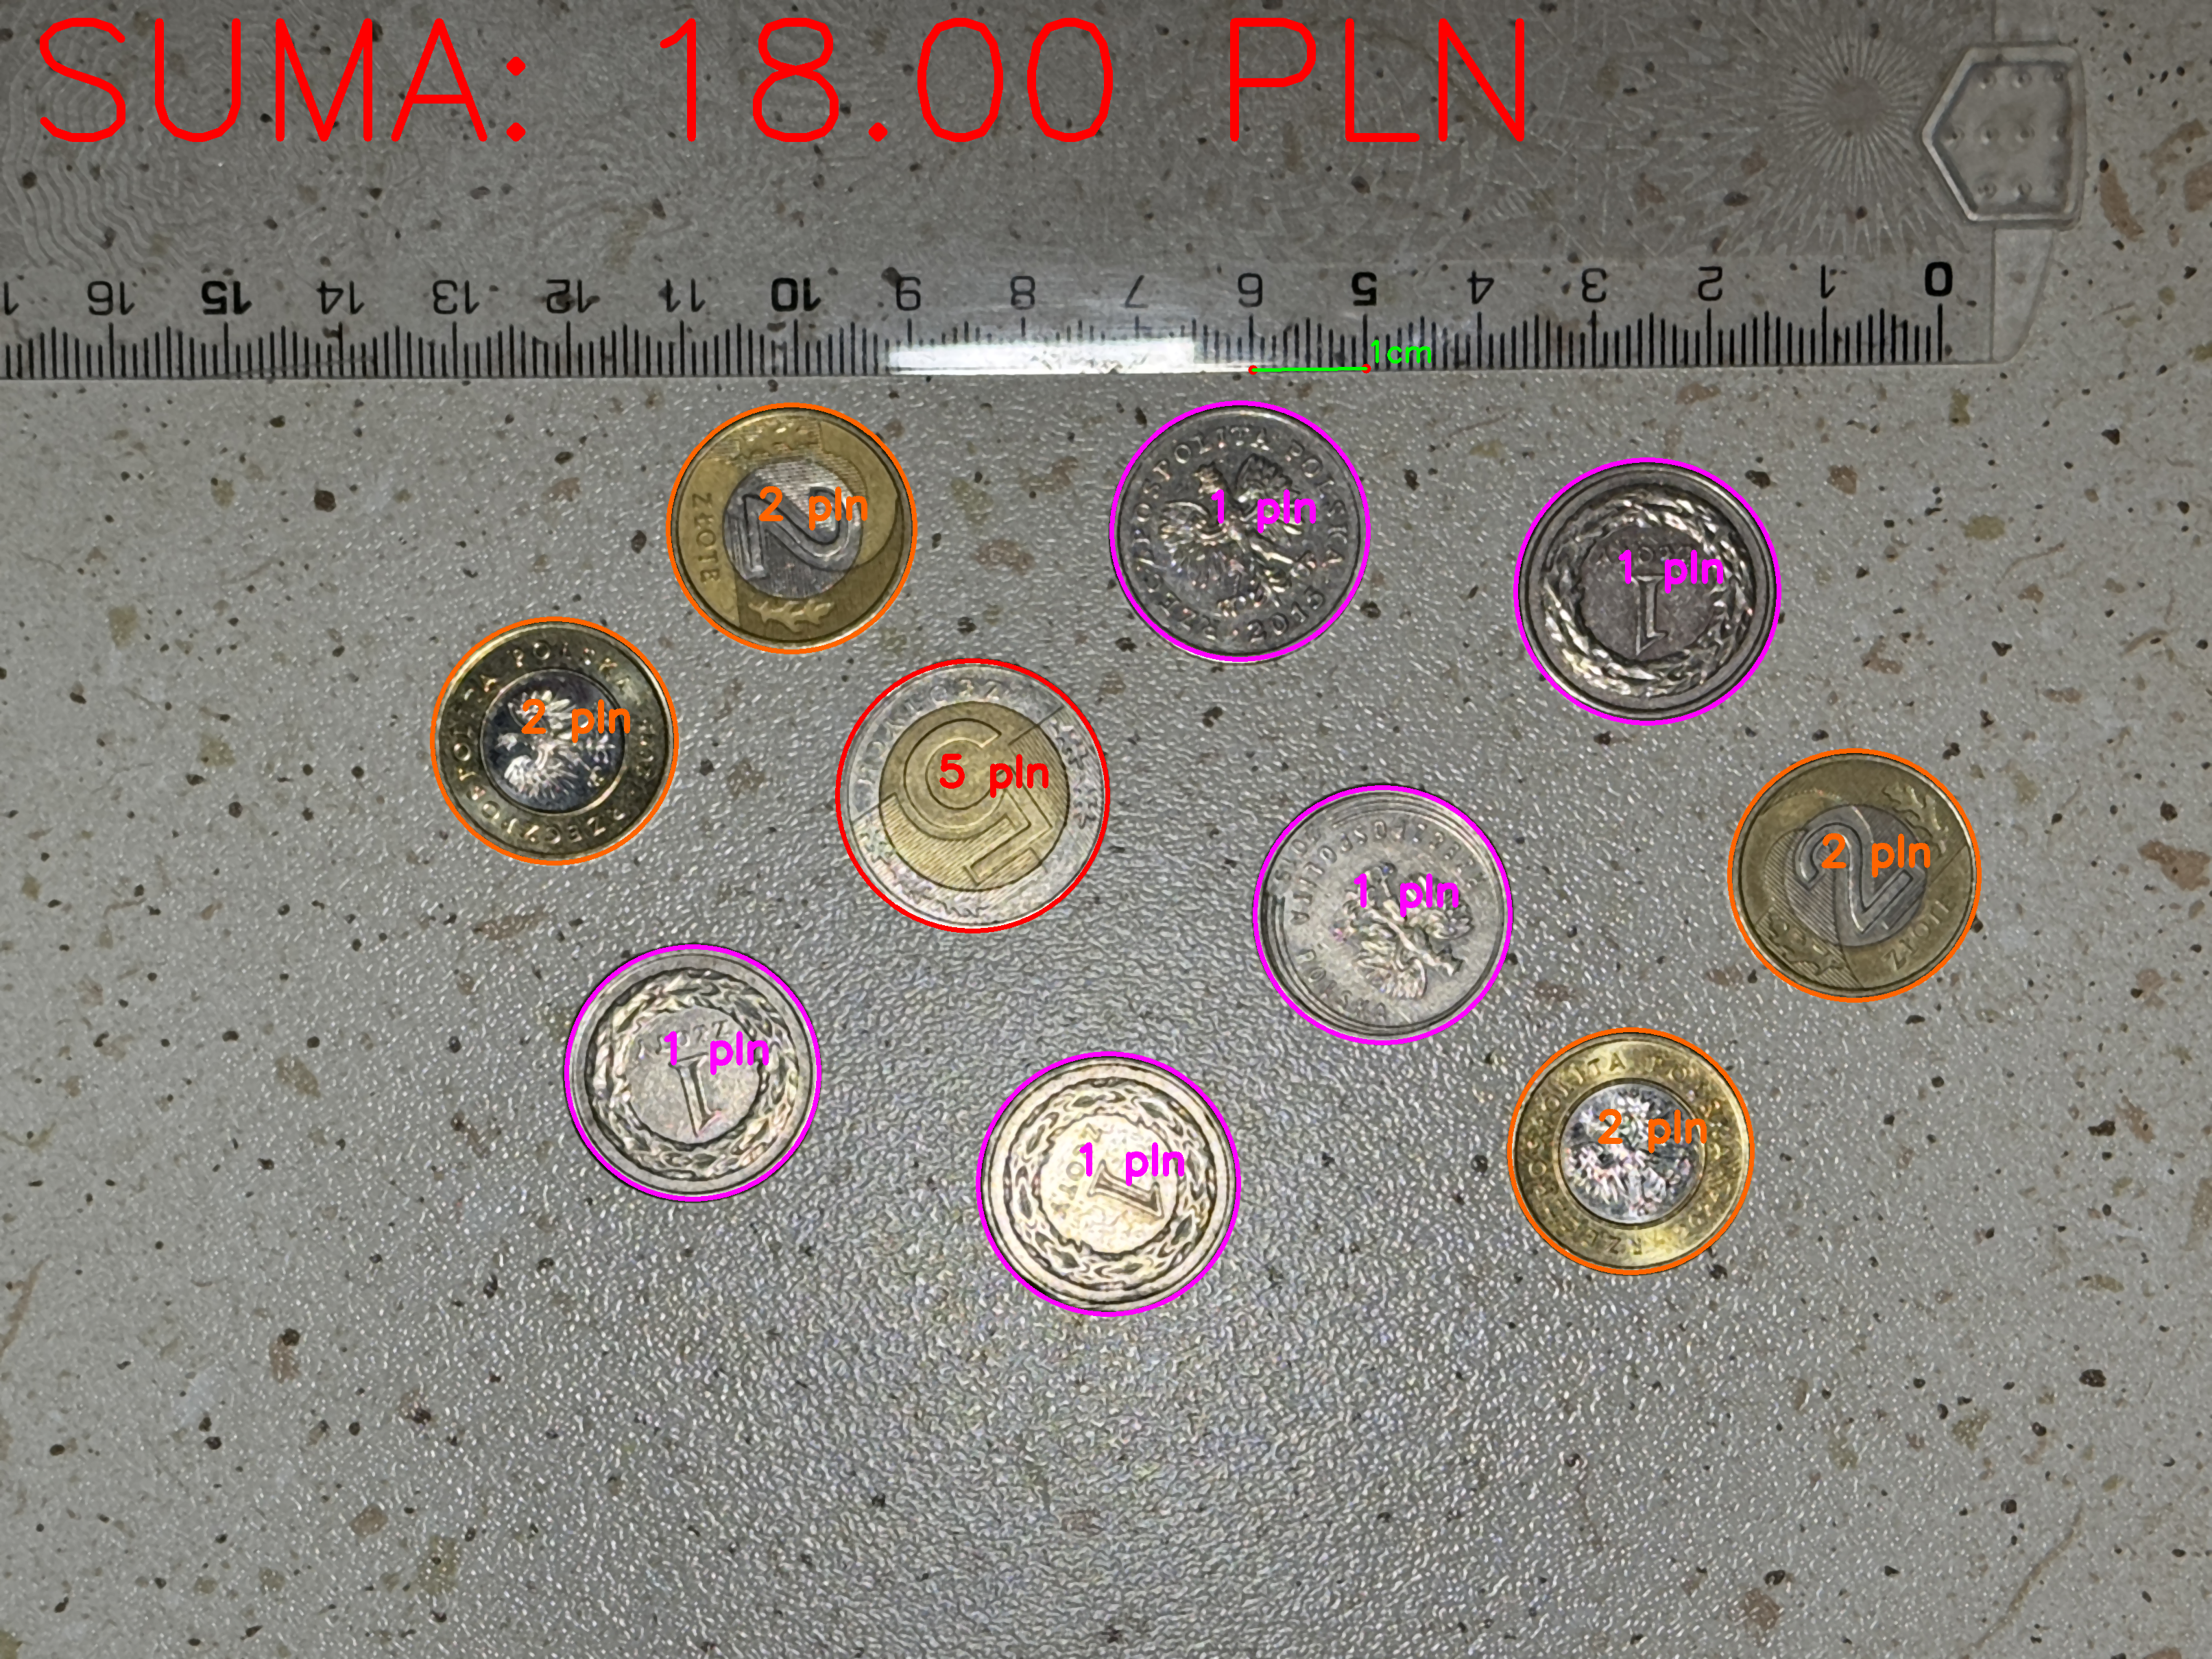
\includegraphics[page=1, width=0.7\textwidth, , trim= 0cm 0cm 0cm 0cm, clip]{wynik_detekcji_blat_dp=1_p1=317_p2=45.png}
    %     \caption{Wyniki detekcji algorytmu dla monet na blacie}
    %     \label{fig:blat}
    % \end{figure}


\subsection{Analiza wyników}

Otrzymane wyniki umieszczono w tabeli~\ref{tab:wyniki}. Dla każdego wariantu badano po pięć zdjęć, skuteczność była oceniania jako ilość poprawnie rozpoznanych monet do wszystkich monet na zdjęciach.

\begin{table}[H]
\caption{Wyniki otrzymanych obrazów}
\label{tab:wyniki}
\centering
\begin{tabular}{|c|c|c|c|c|}
\hline
\textbf{Wariant} & \textbf{Ilość monet} & \textbf{Poprawnie rozpoznanie} & \textbf{Niepoprawnie} & \textbf{Skuteczność [\%]}\\ \hline
Skaner & 65 & 64 & 1 & 98,5\\ \hline
Flesz & 69 & 67 & 2 & 97,1\\ \hline
Biurko & 69 & 60 & 9 & 86,9\\ \hline
\end{tabular}
\end{table}

\subsection{Wnioski}
\begin{itemize}
\item Dokładność systemu jest bezpośrednio zależna od precyzji etapu kalibracji skali. Błędy w zaznaczeniu odcinka referencyjnego 1 cm propagują się do dalszych obliczeń średnicy monet, co bezpośrednio wpływa na poprawność ich klasyfikacji. 
\item Wykorzystanie kanału nasycenia (\textit{HSV}) pozwoliło na skuteczne rozróżnienie monet o zbliżonych średnicach (1~PLN vs 2~PLN). Średnie nasycenie dla monet bimetalicznych (2~PLN i 5~PLN) było stabilnie wyższe o około 15--20 jednostek w skali OpenCV względem monet miedzioniklowych, co stanowiło wiarygodny deskryptor weryfikujący. 
\item Działanie programu kalibracyjnego znacząco upraszcza dobór prawidłowych nastaw dla danego wariantu oświetleniowego, jednak kluczową rolę odgrywa odpowiednie przygotowanie wstępne zdjęć (preprocessing). 
\item Największy wpływ na skuteczność detekcji okręgów w algorytmie Hougha miała regulacja parametru \texttt{Param1}, odpowiedzialnego za detekcję krawędzi metodą Canny’ego. Pozostałe parametry mogły pozostać na stałym poziomie, co wskazuje na dominującą rolę jakości krawędzi w procesie wykrywania obiektów. 
\item Zdjęcia wykonane na skanerze oraz przy użyciu lampy błyskowej cechują się znacznie wyższą skutecznością w porównaniu do zdjęć wykonanych na biurku bez doświetlenia scenerii światłem o dużym natężeniu. 
\item Na zdjęciach wykonanych na biurku widoczne są zniekształcenia przy krawędziach obrazu wynikające z krzywizny soczewki (dystorsja). Wpływa to na błędną identyfikację monet umieszczonych blisko brzegu kadru. 
\item Ważnym czynnikiem wpływającym na skuteczność algorytmu jest unifikacja sposobu wykonywania zdjęć. W przypadku fotografii mobilnej warto rozważyć użycie statywu; w niniejszym projekcie stabilizację warunków zapewniono poprzez wyznaczenie obszaru roboczego na powierzchni biurka przy użyciu czarnej taśmy i określenia poziomego położenia telefonu, pokazywanego w aplikacji aparatu. 
\item W przypadku monet groszowych nie uzyskano zadowalającej skuteczności rozpoznawania, głównie ze względu na niewielkie różnice w ich średnicach oraz większą podatność na zakłócenia detekcji. Z tego powodu nominały te zostały świadomie pominięte w finalnej wersji systemu.

\end{itemize}


\section{Podsumowanie}
W ramach projektu zaprojektowano i zaimplementowano system wizyjny służący do przeliczania wartości polskich monet (1, 2 oraz 5 PLN). Kluczowym osiągnięciem było stworzenie stabilnego potoku przetwarzania, który łączy klasyczną geometrię (transformata Hougha) z analizą barwną w przestrzeni HSV.


\end{document}